\documentclass[tikz, border=15pt]{standalone}
\usepackage{helvet}
\renewcommand{\familydefault}{\sfdefault} % Modern sans-serif font
\usetikzlibrary{positioning, fit, backgrounds, shapes.geometric, arrows.meta, calc}

\begin{document}
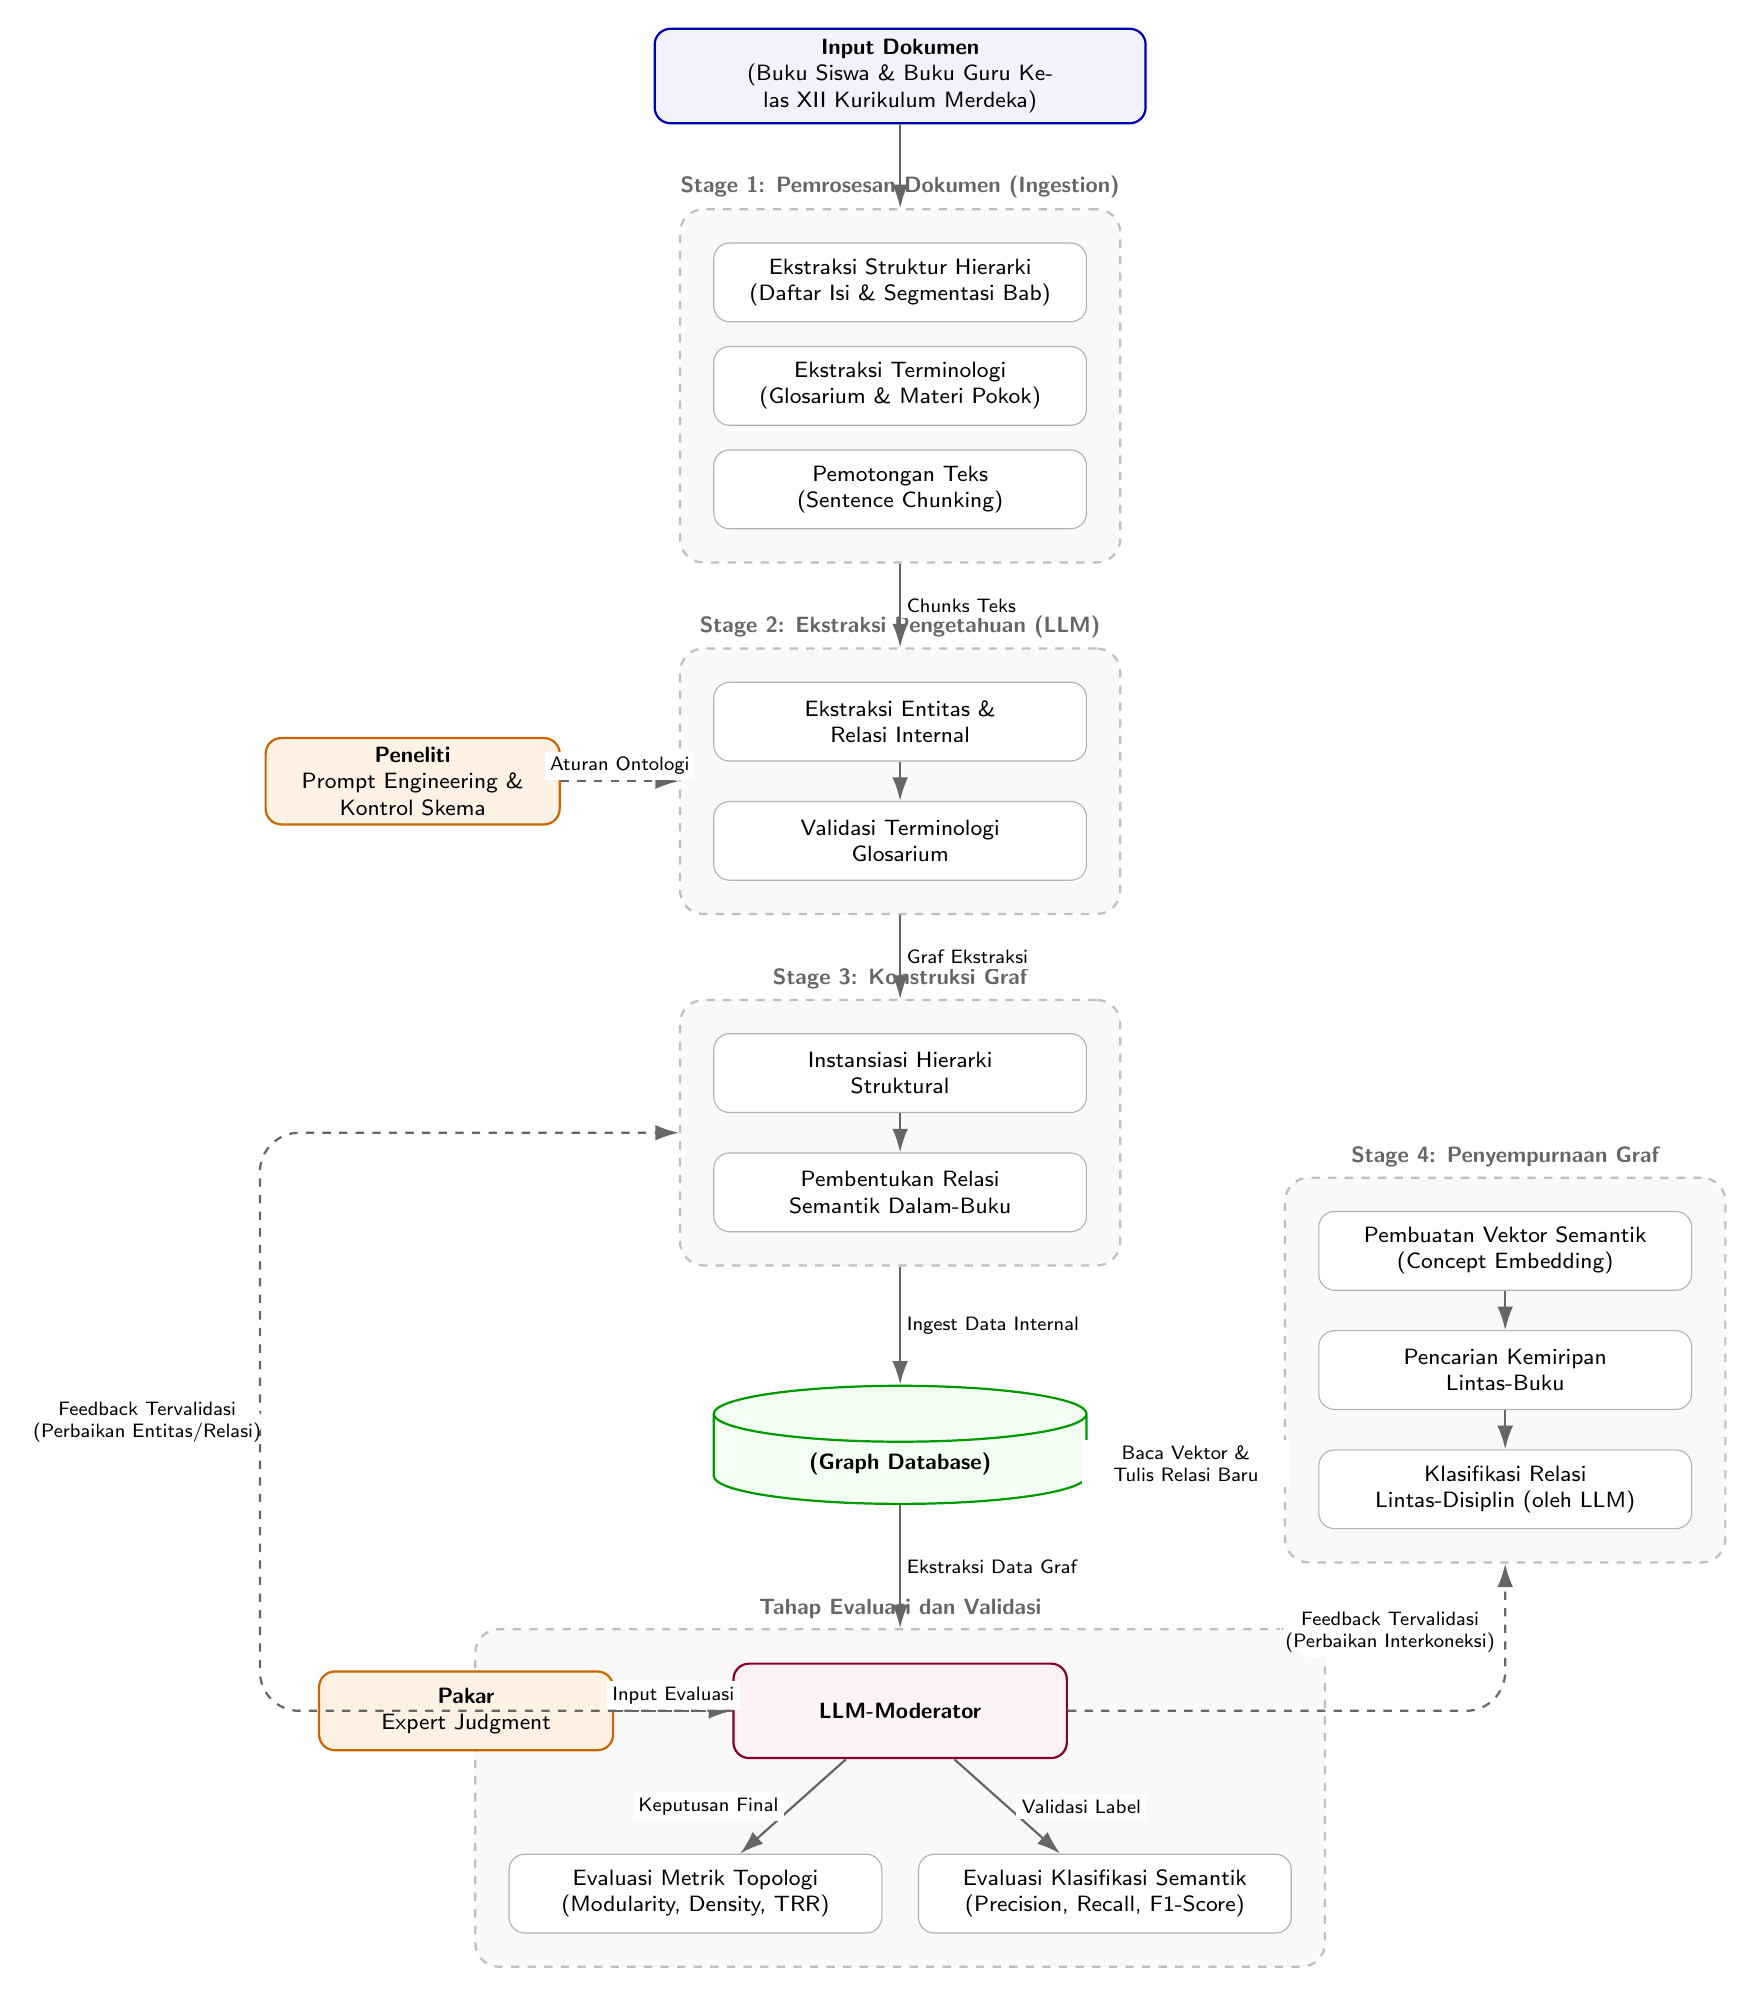
\begin{tikzpicture}[
    % ==== STYLE DEFINITIONS ====
    node distance=1.2cm and 1.5cm,
    font=\small,
    % Node Styles
    basic/.style={draw, text centered, font=\footnotesize, minimum height=1cm, rounded corners=2mm, text width=4.5cm},
    input/.style={basic, fill=blue!5, thick, draw=blue!70!black, text width=6cm, minimum height=1.2cm},
    process/.style={basic, fill=white, draw=gray!60},
    db/.style={basic, fill=green!5, cylinder, shape border rotate=90, aspect=0.15, text width=4.5cm, minimum height=1.5cm, thick, draw=green!60!black, rounded corners=0mm},
    human/.style={basic, fill=orange!10, thick, draw=orange!80!black, text width=3.5cm},
    llmmod/.style={basic, fill=purple!5, thick, draw=purple!70!black, text width=4cm, minimum height=1.2cm},
    % Subgraph/Box Styles
    stagebox/.style={draw, gray!50, thick, dashed, rounded corners=3mm, fill=gray!5, inner sep=12pt},
    % Arrow Styles
    arrow/.style={thick, -{Latex[length=3mm, width=2mm]}, draw=gray!80!black},
    darrow/.style={thick, dashed, -{Latex[length=3mm, width=2mm]}, draw=gray!80!black},
    doublearrow/.style={thick, <->, >=stealth, draw=gray!80!black}
]

    % ==== 1. INPUT ====
    \node[input] (input) {\textbf{Input Dokumen}\\(Buku Siswa \& Buku Guru Kelas XII Kurikulum Merdeka)};

    % ==== 2. STAGE 1 ====
    \node[process, below=1.5cm of input] (a1) {Ekstraksi Struktur Hierarki\\(Daftar Isi \& Segmentasi Bab)};
    \node[process, below=0.3cm of a1] (a2) {Ekstraksi Terminologi\\(Glosarium \& Materi Pokok)};
    \node[process, below=0.3cm of a2] (a3) {Pemotongan Teks\\(Sentence Chunking)};
    
    \begin{scope}[on background layer]
        \node[stagebox, fit=(a1)(a2)(a3), label={[font=\bfseries\footnotesize, text=gray!80!black]above:Stage 1: Pemrosesan Dokumen (Ingestion)}] (stage1) {};
    \end{scope}

    \draw[arrow] (input) -- (stage1);

    % ==== 3. STAGE 2 ====
    \node[process, below=1.5cm of stage1] (b1) {Ekstraksi Entitas \&\\Relasi Internal};
    \node[process, below=0.5cm of b1] (b2) {Validasi Terminologi\\Glosarium};
    
    \begin{scope}[on background layer]
        \node[stagebox, fit=(b1)(b2), label={[font=\bfseries\footnotesize, text=gray!80!black]above:Stage 2: Ekstraksi Pengetahuan (LLM)}] (stage2) {};
    \end{scope}

    \draw[arrow] (b1) -- (b2);
    \draw[arrow] (stage1) -- node[right, font=\scriptsize, fill=white, inner sep=2pt] {Chunks Teks} (stage2);

    % ==== 4. HUMAN INTERVENTION 1 ====
    \node[human, left=1.5cm of stage2] (human1) {\textbf{Peneliti}\\Prompt Engineering \&\\Kontrol Skema};
    \draw[darrow] (human1) -- node[above, font=\scriptsize, fill=white, inner sep=2pt] {Aturan Ontologi} (stage2);

    % ==== 5. STAGE 3 ====
    \node[process, below=1.5cm of stage2] (c1) {Instansiasi Hierarki\\Struktural};
    \node[process, below=0.5cm of c1] (c2) {Pembentukan Relasi\\Semantik Dalam-Buku};
    
    \begin{scope}[on background layer]
        \node[stagebox, fit=(c1)(c2), label={[font=\bfseries\footnotesize, text=gray!80!black]above:Stage 3: Konstruksi Graf}] (stage3) {};
    \end{scope}

    \draw[arrow] (c1) -- (c2);
    \draw[arrow] (stage2) -- node[right, font=\scriptsize, fill=white, inner sep=2pt] {Graf Ekstraksi} (stage3);

    % ==== 6. DATABASE ====
    \node[db, below=1.5cm of stage3] (db) {\textbf{(Graph Database)}};
    \draw[arrow] (stage3) -- node[right, font=\scriptsize, fill=white, inner sep=2pt] {Ingest Data Internal} (db);

    % ==== 7. STAGE 4 ====
    % Positioned to the right of the DB to balance the layout vertically
    \node[process, right=2.5cm of stage3, yshift=-1.5cm] (d1) {Pembuatan Vektor Semantik\\(Concept Embedding)};
    \node[process, below=0.5cm of d1] (d2) {Pencarian Kemiripan\\Lintas-Buku};
    \node[process, below=0.5cm of d2] (d3) {Klasifikasi Relasi\\Lintas-Disiplin (oleh LLM)};
    
    \begin{scope}[on background layer]
        \node[stagebox, fit=(d1)(d2)(d3), label={[font=\bfseries\footnotesize, text=gray!80!black]above:Stage 4: Penyempurnaan Graf}] (stage4) {};
    \end{scope}

    \draw[arrow] (d1) -- (d2);
    \draw[arrow] (d2) -- (d3);
    
    \draw[doublearrow] (db.east) -- node[fill=white, text width=2.5cm, align=center, font=\scriptsize, inner sep=2pt] {Baca Vektor \&\\Tulis Relasi Baru} (stage4.west |- db.east);

    % ==== 8. EVALUATION ====
    \node[llmmod, below=2cm of db] (e3) {\textbf{LLM-Moderator}};
    \node[process, below=1.2cm of e3, xshift=-2.6cm] (e1) {Evaluasi Metrik Topologi\\(Modularity, Density, TRR)};
    \node[process, below=1.2cm of e3, xshift=2.6cm] (e2) {Evaluasi Klasifikasi Semantik\\(Precision, Recall, F1-Score)};
    
    \begin{scope}[on background layer]
        \node[stagebox, fit=(e3)(e1)(e2), label={[font=\bfseries\footnotesize, text=gray!80!black]above:Tahap Evaluasi dan Validasi}] (eval) {};
    \end{scope}

    \draw[arrow] (db) -- node[right, font=\scriptsize, fill=white, inner sep=2pt] {Ekstraksi Data Graf} (eval);
    \draw[arrow] (e3) -- node[left, font=\scriptsize, xshift=-0.1cm, fill=white, inner sep=2pt] {Keputusan Final} (e1);
    \draw[arrow] (e3) -- node[right, font=\scriptsize, xshift=0.1cm, fill=white, inner sep=2pt] {Validasi Label} (e2);

    % ==== 9. HUMAN INTERVENTION 2 ====
    \node[human, left=1.5cm of e3] (human2) {\textbf{Pakar}\\Expert Judgment};
    \draw[darrow] (human2) -- node[above, font=\scriptsize, fill=white, inner sep=2pt] {Input Evaluasi} (e3);

    % ==== 10. FEEDBACK LOOPS ====
    % E3 to Stage 3 (Routes far to the left to avoid crossing Human 2)
    \draw[darrow, rounded corners=5mm] 
        (e3.west) -- ++(-6,0) |- 
        node[pos=0.25, left, font=\scriptsize, align=center, fill=white, inner sep=2pt, xshift=1mm] {Feedback Tervalidasi\\(Perbaikan Entitas/Relasi)} 
        (stage3.west);

    % E3 to Stage 4 (Routes out right and up into the bottom of Stage 4)
    \draw[darrow, rounded corners=5mm] 
        (e3.east) -| 
        node[pos=0.25, right, font=\scriptsize, align=center, fill=white, inner sep=2pt, xshift=-1mm, yshift=1cm] {Feedback Tervalidasi\\(Perbaikan Interkoneksi)} 
        (stage4.south);

\end{tikzpicture}
\end{document}